
\subsection{Named Entity Recognition}

This section will go into the details of the Named Entity Recognition task, what
the specifics are, considerations in regards to the data used, any issues we
came across, and the results of our experiments.

\subsubsection{Task definition}

Named Entity Recognition is a classification task of different types of
entities, such as places, people, organisation, times, and more. Entities can
consist of one or more words (and/or numbers), eg.\ ``Eurovision Song Contest
2019'' is a single entity of 3 words and a number. The classifier should
correctly identify the whole entity and not just part of it. We didn't take this
into consideration before running the experiments so our results are on a word
by word basis and doesn't tell us if the whole entity was correctly classified
or not.

The same entity might never show up in the dataset twice so it's important for
the classifier to be able to figure out based on context of the other words in
the sentence if there is an entity or not. It is impossible to simply remember
that a word refers to an entity since the word was most likely not seen during
training.

Usually the performance of a classifier for the NER task is measured by a $F_1$
Score, which considers the classifier's precision and recall. The precision is
the classifier's ability to correctly classify an entity given all attempts, and
recall is the ability to correctly classify an element given how many elements
exists. Say there are 100 entities in a document, the classifier finds 90
entities, 80 of them are correct, 10 of them are wrong, and 20 were not found.
From this we get the precision $P = {80 \over 80 + 10} = 0.88\ldots$, and recall $R
= {80 \over 80 + 20} = 0.8$. The $F_1$ score is simply the harmonic mean between
the precision and recall given by $F_1 = 2 \cdot {precision \cdot recall \over
precision + recall}$. Based on our example this would be $F_1 = 2 \cdot
{0.88 \ldots \cdot 0.8 \over 0.88\ldots + 0.8} = 0.8421$.~\ref{https://www.toyota-ti.ac.jp/Lab/Denshi/COIN/people/yutaka.sasaki/F-measure-YS-26Oct07.pdf}.

The rationale behind using the $F_1$ score is that usually a lot of the data is
non-entities. A classifier which classified nothing as an entity would have a
great accuracy on datasets with few entities. Since we didn't evaluate if whole
entities were classified correctly, we will base our score on the individual
words and the score might therefore be higher than otherwise. Since we aren't
comparing with models outside our own this shouldn't be an issue.


\subsubsection{Data}

For the NER task we used auto-annotated wikipedia data from~\ref{}{Cross-lingual
Name Tagging and Linking for 282 Languages}. As the title suggests, this dataset
contains annotated data for 282 languages in varying sizes. 

The datasets are all in the BIO (or IOB) format, which has three different
entities, organisations, people, and locations. The BIO format uses the
convention that the beginning of an entity is prefixes with a B and the
continuation of an entity is prefixed with an I (for inside). Tokens which are
not part of an entity is labeled O (for other). This gives the 7 labels, B-ORG,
B-PER, B-LOC, I-ORG, I-PER, I-LOC, and O. 

Since all the datasets were created based on wikipedia data we didn't have to
take varying sources into considerations, as was necessary for the POS task.

The data being auto-annotated means it might not be of the same standard as the
POS data. Ideally this shouldn't affect the experiments since the word orderings
are still the same, and systematic errors in the data would hopefully happen for
all languages in the datasets.

For Japanese which doesn't use spaces to differentiate between the beginning and
the end of words, the data is split and labeled character by character, this
differs from the POS data where words are split in a more natural way. This has
an influence on the results and means that Japanese isn't as comparable between
tasks as other languages. Since it turns out that our Polyglot embedding has a
somewhat similar way to split words it can have a positive effect on the
performance.

As the data used for training the model is the same data used for training the
polyglot word embeddings, the models don't have the same kind of variety from
the data as is the case for the POS task. This may result in worse performance
since the models might be more likely to overfit.

A table of the languages with the number of entities in their respective dataset
is given below in table \ref{}.

\subsubsection{Results and analysis}

\begin{figure}[h]
    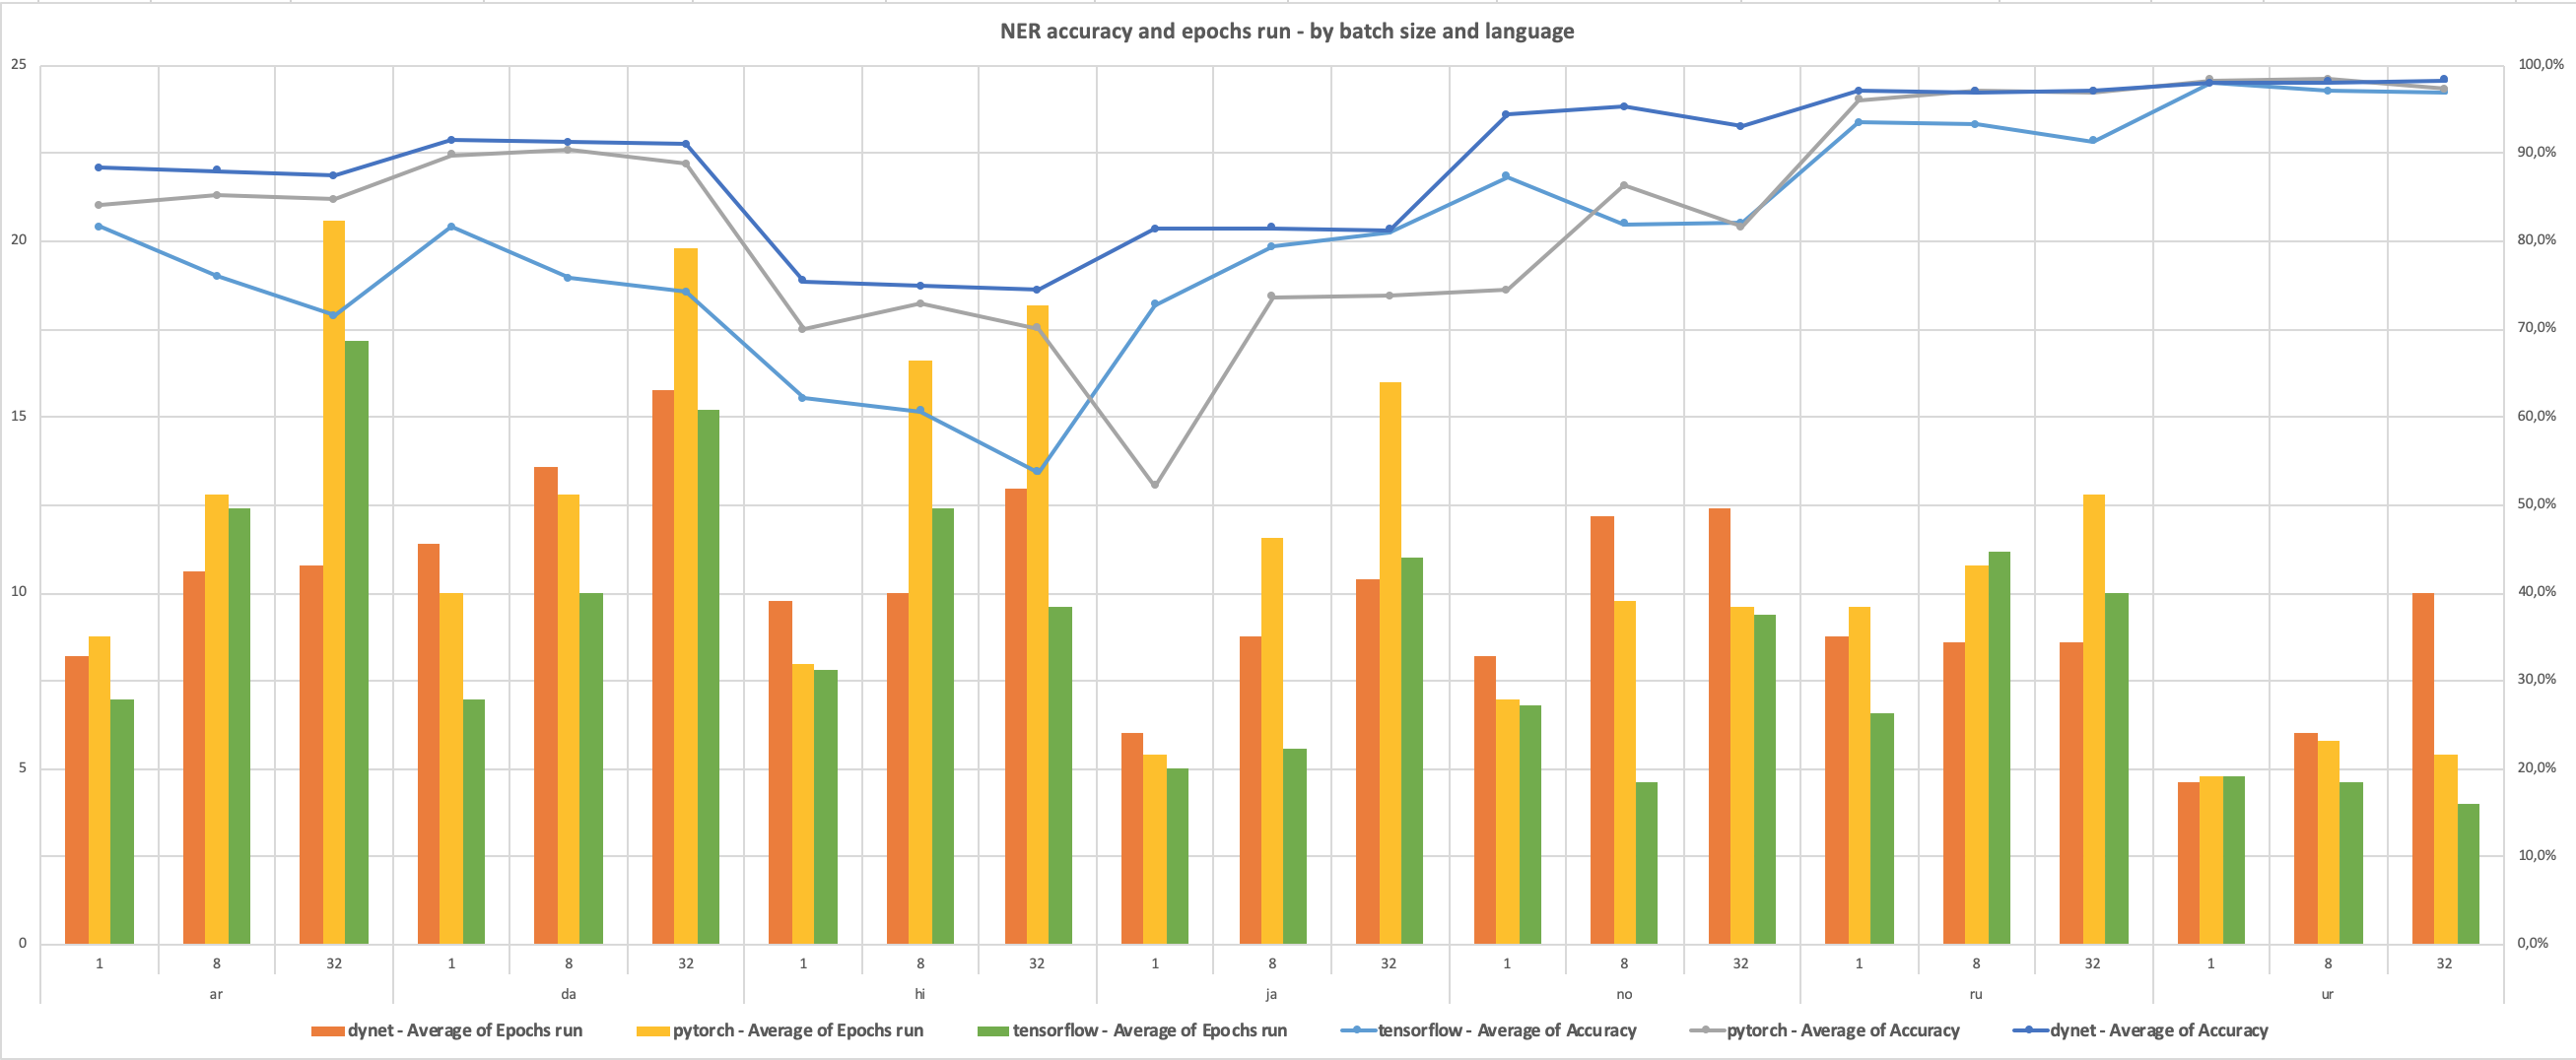
\includegraphics[width=\textwidth]{ner-acc-epo.png}
    \caption{NER accuracy and epochs run --- by batch size and language
    }\label{chart:ner-acc-epo}
\end{figure}


\pagebreak
